\section{任务一}
\subsection{Enigma密码机程序编写}
按照实验指导书的配置设置 Enigma 机的加密代码，本部分在参考程序的基础上进行整理和修改，主要完成以下配置：
\begin{itemize}
    \item 使用 5 条连线的接线板 $S=[AV\ BS\ CG\ MN\ OX]$ 设置密钥 $K_1$；
    \item 使用实验指导书给出的三个转子，按照快速、中速、慢速的顺序设置为 $I$、$II$、$III$，并将起始位置设置为 $K_2=(8,9,10)$；
    \item 设置反射器 $T$。反射器是实验给定的固定部件，不作为本实验中需要恢复的密钥部分。
\end{itemize}

\subsection{测试Enigma密码机}
使用编写完成的 Enigma 机程序加密给定明文 \texttt{WETTER}，输出密文为 \texttt{TWNVCX}，运行结果如下图所示：
\begin{figure}[H]
    \centering
    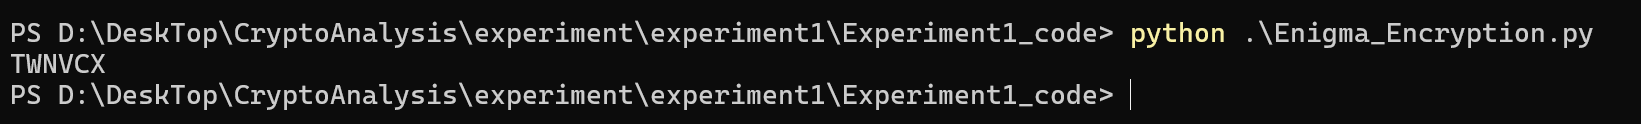
\includegraphics[width = 1\textwidth]{figures/task1_enigma_encryption.png}
    \caption{Enigma机加密测试明文}
\end{figure}
由输出结果可知，程序能够按照实验指导书给定的接线板、转子、反射器和起始位置完成明文加密。
